\documentclass[simplex.tex]{subfiles}
% NO NEED TO INPUT PREAMBLES HERE
% packages are inherited from simplex.tex; you can compile this on its own
\subsection{ndreg}
%
%We received three new CLARITY image volumes from our colleagues at Stanford University. 
%Each dataset contained two channels of a single mouse brain hemisphere at a 585 $\mu m$ $\times$ 585 $\mu m$ $\times$ 5000 $\mu m$ resolution.
%The images were ingested and propagated to lower resolutions using NeuroData infrastructure.
%NeuroData's registration module (ndreg) was then used to register each image to the Allen institute's mouse Reference Atlas (ARA).
%
%First each image was reoriented to the ARA, the background was subtracted and a mask was generated to eliminate bright regions.
%After affine alignment, each Stanford image was deformably aligned to the ARA through Large Deformation Diffeomorphic Metric Mapping (LDDMM).
%Since the ARA and CLARITY images differed greatly in intensity profile, mutual information matching was adopted during this step.
%Alignment was done in a 3-step multi-resolution approach, with registration at coarser scales initializing the alignment at subsequent finer scales.
%It was clear from the ARA-CLARITY checkerboard composite images that registration proceeded successfully (Figure~\ref{fig:ndregAiley}).
%
%\begin{figure}[h!]
%\begin{cframed}
%\centering
%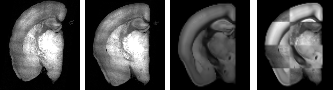
\includegraphics[width=0.75\textwidth]{../../figs/ndreg-ailey.png}
%\caption{
%  Coronal slices from image volumes.
%  From left to right: CLARITY before LDDMM, CLARITY after LDDMM, ARA, checkerboard composite of ARA and CLARITY after LDDMM.
%}
%\label{fig:ndregAiley}
%\end{cframed}
%\end{figure}
%
\end{document}
